\documentclass[tikz,border=1.5pt]{standalone}
\newif\ifko \kofalse

% style.tex — 구성도 공용 (standalone, xelatex). \kotrue / \kofalse 를 먼저 정함.
\usepackage{mathptmx}
\usepackage[no-math]{fontspec}
\setmainfont{TeX Gyre Heros}
\ifko
  \newfontfamily\krfont{Noto Sans CJK KR}[Scale=0.9]
  \usepackage[Latin,Korean]{ucharclasses}
  \setTransitionsForKorean{\begingroup\krfont}{\endgroup}
\fi
\usepackage{xcolor}
\definecolor{cFRiii}{HTML}{0072B2}
\definecolor{cFRv}{HTML}{D55E00}
\definecolor{cEmph}{HTML}{009E73}
\usepackage{tikz}
\usetikzlibrary{positioning,fit,backgrounds,arrows.meta,calc,shapes.geometric,shapes.misc,decorations.pathreplacing}
\newcommand{\T}[2]{\ifko #1\else #2\fi}
\tikzset{
  >={Stealth[length=2.2mm,width=1.6mm]},
  every node/.style={font=\fontsize{7.2}{8.6}\selectfont},
  box/.style={draw=black, line width=0.5pt, rounded corners=1.2pt, fill=white, align=center, inner sep=2.6pt, minimum height=8.5mm, text width=#1},
  box/.default=24mm,
  gbox/.style={box=#1, fill=black!6},
  gbox/.default=24mm,
  ebox/.style={box=#1, draw=cEmph, line width=1.0pt, fill=cEmph!7},
  ebox/.default=24mm,
  grp/.style={draw=black!55, dashed, line width=0.45pt, rounded corners=2pt, inner sep=3.2mm},
  grplabel/.style={anchor=north west, font=\fontsize{7.6}{9}\selectfont\bfseries, inner sep=1.2pt, fill=white},
  ar/.style={->, line width=0.6pt},
  ear/.style={->, line width=1.1pt, draw=cEmph},
  dar/.style={->, line width=0.55pt, dashed},
  small/.style={font=\fontsize{6.3}{7.4}\selectfont},
  lab/.style={font=\fontsize{6.3}{7.4}\selectfont, fill=white, inner sep=1pt},
}
\newcommand{\D}{\fontsize{6.3}{7.5}\selectfont\color{black!78}}
\newcommand{\code}[1]{\texttt{#1}}

\begin{document}
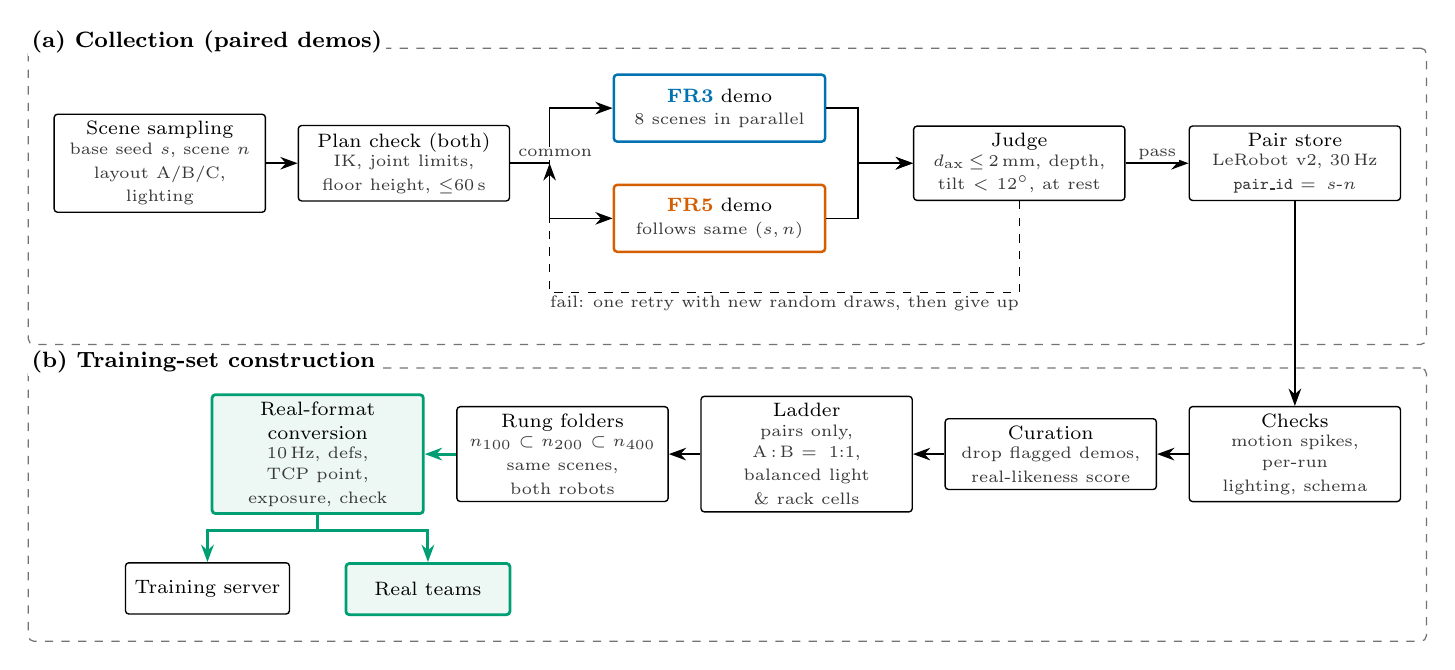
\begin{tikzpicture}[node distance=4mm]
\def\W{25mm}
% ---------------- 1줄: 수집
\node[box=\W, anchor=north west] (s1) at (0,0) {\T{장면 뽑기}{Scene sampling}\\[-0.5pt]{\D\T{기본 시드 $s$, 장면 번호 $n$\\배치 A $\cdot$ B $\cdot$ C, 조명}{base seed $s$, scene $n$\\layout A/B/C, lighting}}};
\node[box=\W, right=of s1] (s2) {\T{두 로봇 계획 확인}{Plan check (both)}\\[-0.5pt]{\D\T{역기구학, 관절 한계,\\바닥 높이, 60 s 이내}{IK, joint limits,\\floor height, $\le$60\,s}}};
\node[box=\W, right=13mm of s2, yshift=7mm, draw=cFRiii, line width=0.9pt] (r3) {\textcolor{cFRiii}{\textbf{FR3}} \T{시연}{demo}\\[-0.5pt]{\D\T{장면 8개 동시}{8 scenes in parallel}}};
\node[box=\W, right=13mm of s2, yshift=-7mm, draw=cFRv, line width=0.9pt] (r5) {\textcolor{cFRv}{\textbf{FR5}} \T{시연}{demo}\\[-0.5pt]{\D\T{같은 $(s, n)$ 따라가기}{follows same $(s, n)$}}};
\node[box=\W, right=11mm of r3, yshift=-7mm] (j) {\T{판정}{Judge}\\[-0.5pt]{\D $d_{\mathrm{ax}}\!\le\!2$\,mm, \T{깊이}{depth},\\\T{기울기}{tilt} $<12^\circ$, \T{멈춤}{at rest}}};
\node[box=\W, right=8mm of j] (st) {\T{짝 저장}{Pair store}\\[-0.5pt]{\D LeRobot v2, 30\,Hz\\\code{pair\_id} $= s$-$n$}};
\draw[ar] (s1) -- (s2);
\coordinate (fork) at ($(s2.east)+(5mm,0)$);
\draw[ar] (s2.east) -- (fork) |- (r3.west);
\node[lab, anchor=south west, xshift=0.6mm, yshift=0.4mm] at (s2.east) {\D\T{둘 다 됨}{common}};
\draw[ar] (fork) |- (r5.west);
\draw[ar] (r3.east) -- ++(4mm,0) |- (j.west);
\draw[ar] (r5.east) -- ++(4mm,0) |- (j.west);
\draw[ar] (j) -- node[lab, above]{\D\T{성공}{pass}} (st);
\coordinate (rt) at ($(j.south |- r5.south)+(0,-5mm)$);
\draw[dar] (j.south) -- (rt) -- node[lab, below]{\D\T{실패: 새 무작위 값으로 한 번 더 (그래도 실패면 포기)}{fail: one retry with new random draws, then give up}} (fork |- rt) -- (fork);
% ---------------- 2줄: 다듬기
\node[box=\W, anchor=north east] (c1) at ($(st.south east)+(0,-26mm)$) {\T{점검}{Checks}\\[-0.5pt]{\D\T{움직임 튐, 실행별 조명,\\형식 점검}{motion spikes, per-run\\lighting, schema}}};
\node[box=\W, left=of c1] (c2) {\T{선별}{Curation}\\[-0.5pt]{\D\T{표시된 시연 빼기,\\실물 닮음 점수}{drop flagged demos,\\real-likeness score}}};
\node[box=\W, left=of c2] (c3) {\T{사다리}{Ladder}\\[-0.5pt]{\D\T{짝만, A\,:\,B $=1{:}1$,\\조명 $\cdot$ 랙 칸 고르게}{pairs only, A\,:\,B $=1{:}1$,\\balanced light \& rack cells}}};
\node[box=\W, left=of c3] (c4) {\T{칸 폴더}{Rung folders}\\[-0.5pt]{\D $n_{100} \subset n_{200} \subset n_{400}$\\\T{두 로봇 같은 장면}{same scenes, both robots}}};
\node[ebox=\W, left=of c4] (c5) {\T{실물 형식 변환}{Real-format conversion}\\[-0.5pt]{\D\T{10 Hz, 정의 $\cdot$ 기준점,\\노출, 점검}{10\,Hz, defs, TCP point,\\exposure, check}}};
\draw[ar] (st.south) -- (c1.north);
\draw[ar] (c1) -- (c2); \draw[ar] (c2) -- (c3); \draw[ar] (c3) -- (c4); \draw[ear] (c4) -- (c5);
\node[box=19mm, minimum height=6.5mm, below=6mm of c5, xshift=-14mm] (o1) {\T{학습 서버}{Training server}};
\node[ebox=19mm, minimum height=6.5mm, below=6mm of c5, xshift=14mm] (o2) {\T{실물 팀}{Real teams}};
\draw[ear] (c5.south) -- ++(0,-2mm) -| (o1.north);
\draw[ear] (c5.south) -- ++(0,-2mm) -| (o2.north);
\begin{scope}[on background layer]
\coordinate (rtl) at ($(rt)+(0,-3.4mm)$);
\node[grp, fit=(s1)(s2)(r3)(r5)(st)(rtl)] (GA) {};
\coordinate (bl) at (s1.west |- o1.south);
\node[grp, fit=(c1)(c5)(o1)(o2)(bl)] (GB) {};
\end{scope}
\node[grplabel] at ($(GA.north west)+(0,2.6mm)$) {(a) \T{수집 (짝 시연)}{Collection (paired demos)}};
\node[grplabel] at ($(GB.north west)+(0,2.6mm)$) {(b) \T{학습 데이터 만들기}{Training-set construction}};
\end{tikzpicture}
\end{document}
